\chapter{伊辛关联、平均场与自发磁化}

\lectureoverview{一维伊辛链可以通过将格点自旋替换为键变量来精确求解。这一变量替换把配分函数变成一个乘积，并表明所有有限温度下的关联都按指数衰减。高维点阵的行为则不同，因为每个自旋都从许多近邻接收信息。把它们的联合影响当作一个平均场来处理，就得到一个自洽方程、一个平均场临界温度，以及关于任意小的外场如何选定一个磁化相的精确说明。}

\section{伊辛实际发现了什么}

历史要点应当准确陈述。恩斯特·伊辛求解了威廉·楞次交给他的一维模型，并正确地发现不存在有限温度相变。过分之处在于推断同一结论应当在所有维度都成立。事实并非如此。二维模型已经具有有序的低温相。

高维的精确解对于当前目的来说过于雄心勃勃。一个物理上透明的近似就足以在每个自旋有许多近邻时揭示相变。然而，在作此近似之前，值得先精确求解一维链。精确的一维答案与高维近似之间的对比，指出了维数为一时所缺少的机制。

这里的相变不只是已有偏好逐渐增强。当温度越过一个临界值时，平衡态获得了一种新的宏观性质：即使用来使样品取向的外场已被撤去，非零磁化仍能持续存在。因此，计算必须回答两个彼此独立的问题。一个远处的自旋是否记得某个选定自旋的取向，以及一个无穷小的场能否组织起任意大的样品？

\section{单个自旋作为可复用的构建单元}

取一个二态变量
\begin{equation}
\sigma=\pm1,
\end{equation}
并选择能量约定
\begin{equation}
E(\sigma)=-J\sigma,
\qquad J>0.
\end{equation}
于是态\(\sigma=+1\)具有较低的能量。参数\(J\)可以代表磁矩乘以外加场，但在此计算中只有其乘积进入。

把这个自旋看作与其余一切处于热平衡的小子系统。其配分函数为
\begin{align}
z
&=\sum_{\sigma=\pm1}e^{-\beta E(\sigma)}
 =\sum_{\sigma=\pm1}e^{\beta J\sigma} \\
&=e^{\beta J}+e^{-\beta J}
 =2\cosh(\beta J).
\end{align}

同一结果也可以嵌入到\(N\)个独立自旋的集合中。完整配分函数将简单地是\(Z=z^N\)，因此\(\log Z=N\log z\)，而每个广延热力学量都将是其单自旋值的\(N\)倍。这种子系统观点取代了关于有多少自旋朝上、多少朝下的较长组合计数，但它包含同样的信息。
平均能量由对数导数给出：
\begin{align}
\expect{E}
&=-\frac{\partial}{\partial\beta}\log z \\
&=-J\frac{\sinh(\beta J)}{\cosh(\beta J)}
 =-J\tanh(\beta J).
\end{align}
由于\(E=-J\sigma\)，
\begin{equation}
\expect{\sigma}=\tanh(\beta J).
\end{equation}

\begin{figure}[ht]
\centering
\includegraphics[width=0.80\textwidth]{lecture_09_figure_02.png}
\caption{化为双曲正切形式的单自旋能量与磁化。}
\lectureframe{00:10:06}
\end{figure}

这一个公式包含了两个温度极限。在低温下，\(\beta J\gg1\)，自旋几乎必然处于较低能量的态。在高温下，\(\beta J\ll1\)，所以
\begin{equation}
\expect{\sigma}\simeq \beta J\longrightarrow0.
\end{equation}
热骚动抹去了能量偏好。

\begin{classroomqa}
\audiencequestion{平均能量应当带负号吗？}
\lecturerresponse{是的。热力学恒等式是\(\expect{E}=-\partial_\beta\log z\)，所以结果是\(-J\tanh(\beta J)\)。再除以\(E=-J\sigma\)中的因子\(-J\)，就得到正的磁化\(\expect{\sigma}=\tanh(\beta J)\)。\lecturetimestamp{00:09:15--00:09:44}}
\end{classroomqa}

\section{一维链}

把\(N\)个自旋放在一条开链上，并让相邻自旋相互作用：
\begin{equation}
H=-J\sum_{i=1}^{N-1}\sigma_i\sigma_{i+1},
\qquad \sigma_i=\pm1.
\label{eq:ising-chain}
\end{equation}
对于\(J>0\)，平行的一对贡献\(-J\)，而反平行的一对贡献\(+J\)。因此两个基态是
\begin{equation}
(+,+,\ldots,+)
\qquad\text{and}\qquad
(-,-,\ldots,-).
\end{equation}

\begin{figure}[ht]
\centering
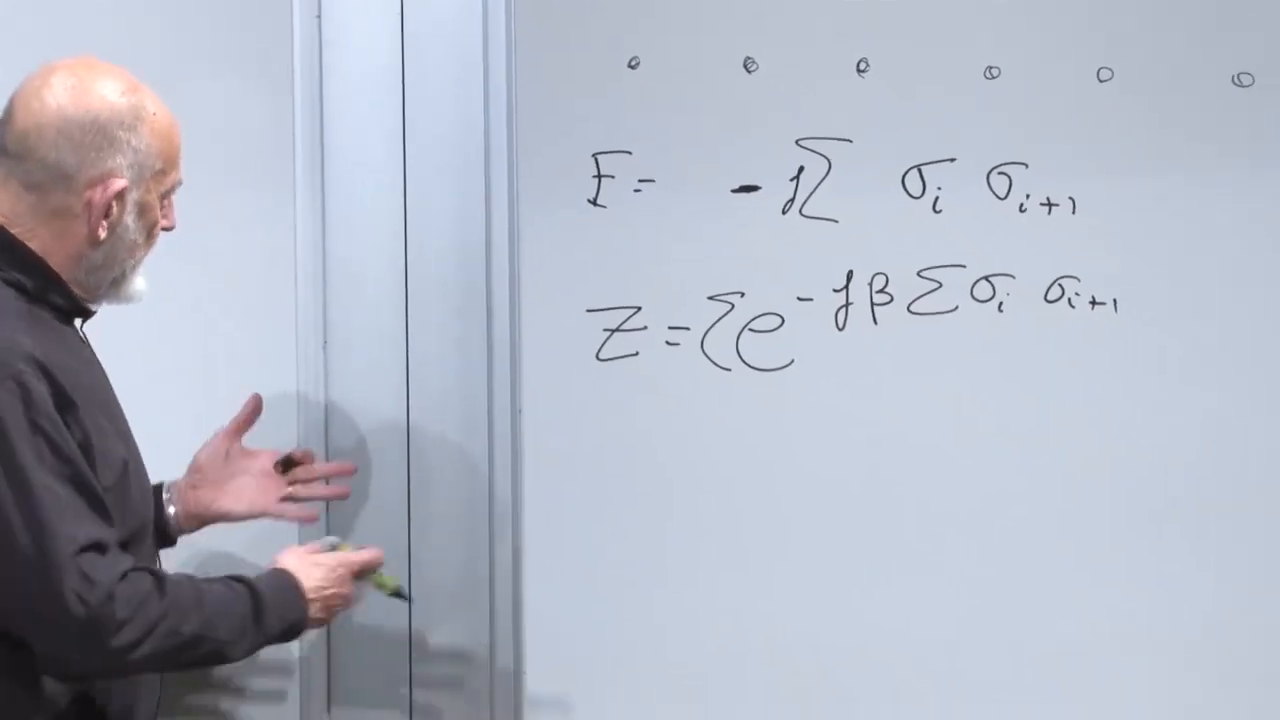
\includegraphics[width=0.80\textwidth]{lecture_09_figure_03.png}
\caption{开链哈密顿量及其玻尔兹曼求和。}
\lectureframe{00:19:15}
\end{figure}

把\(J\)改为\(-J\)会偏好交替自旋。在开链上，或在偶数周期链上，重新定义
\begin{equation}
\widetilde{\sigma}_i=(-1)^i\sigma_i
\end{equation}
把反铁磁符号映射回铁磁符号。这一区别是物理的，但一维配分函数的代数运算相同。奇数周期链是熟悉的例外，因为它无法在不产生阻挫的情况下交替。

\begin{classroomqa}
\audiencequestion{链的哈密顿量中有外磁场吗？}
\lecturerresponse{还没有。式~\eqref{eq:ising-chain}只包含最近邻耦合。均匀外场稍后将作为一个单独的项\(-h\sum_i\sigma_i\)加入，正是为了检验有序态如何响应任意小的偏置。\lecturetimestamp{00:18:54--00:19:13}}
\end{classroomqa}

\subsection{作为关联函数的记忆}

假设已知\(\sigma_i\)处于向上态。这一信息是否会影响相隔\(r\)个键的自旋？诊断量为
\begin{equation}
C(r)=\expect{\sigma_i\sigma_{i+r}}.
\end{equation}
若当\(r\to\infty\)时\(C(r)\)趋于一个非零数，则系统保留长程记忆。若它趋于零，则第一个自旋的影响最终消失。

传话游戏给出了正确的直觉。每个人向下一个人传递一个二进制符号。若每次传递都完美无误，初始比特将无限期地存留下去。若每一步都有任何非零的错误概率，反复传递最终会丢失原始信息。零温度是伊辛链的完美传递极限。任何正温度都允许相邻自旋之间偶尔出现不一致。

为了给出一个数值图像，假设单次传递的保真度为\(0.99\)。两次完美传递发生的概率为\(0.99^2=0.9801\)，而每增加一步就再提供一个因子\(0.99\)。一百步就已经使错误变得常见；一万步则抹去实际意义上的记忆。伊辛链使用的是保真度的带符号度量，而非这种无错误概率，但乘性损失是同样的思想。

在区分概率与关联之后，这个类比就变得精确了。若\(p\)是相邻自旋一致的概率，则
\begin{equation}
\expect{\sigma_i\sigma_{i+1}}
=p-(1-p)=2p-1.
\end{equation}
因此，逐键相乘的量是超额保真度\(2p-1\)，而不是\(p\)本身。

\section{键变量与精确配分函数}

决定性的变量替换是描述关系而非单个自旋：
\begin{equation}
\mu_i=\sigma_i\sigma_{i+1},
\qquad i=1,\ldots,N-1.
\label{eq:bond-variable}
\end{equation}
每个键变量在一致时为\(+1\)，在不一致时为\(-1\)。若固定第一个自旋，则这些键决定之后每一个自旋：
\begin{align}
\sigma_2&=\sigma_1\mu_1,\\
\sigma_3&=\sigma_1\mu_1\mu_2,\\
\sigma_{r+1}&=\sigma_1\prod_{k=1}^{r}\mu_k.
\end{align}
这里没有冗余。数据\((\sigma_1,\mu_1,\ldots,\mu_{N-1})\)等价于\((\sigma_1,\ldots,\sigma_N)\)。

在这些变量下，能量简单地成为
\begin{equation}
H=-J\sum_{i=1}^{N-1}\mu_i.
\end{equation}
原本相互作用的格点变量已变成相互独立的键变量。先对\(\sigma_1\)的两个取值求和，得到
\begin{align}
Z_N
&=2\sum_{\{\mu_i=\pm1\}}
\exp\left(\beta J\sum_{i=1}^{N-1}\mu_i\right)\\
&=2\prod_{i=1}^{N-1}
\left(\sum_{\mu_i=\pm1}e^{\beta J\mu_i}\right)\\
&=2\left[2\cosh(\beta J)\right]^{N-1}.
\label{eq:chain-partition}
\end{align}
共有\(N-1\)个因子，因为含\(N\)个格点的开链有\(N-1\)个键。

前面的因子二来自第一个自旋的全局选择。它对\(\log Z_N\)只贡献\(\log2\)，而键则贡献一个正比于\(N-1\)的项。该因子对于精确的有限尺寸计数很重要，但当\(N\to\infty\)时它从自由能密度中消失。这就是为什么板书可以说它“没什么大不了”，而实际上并没有把它丢弃。

\begin{figure}[ht]
\centering
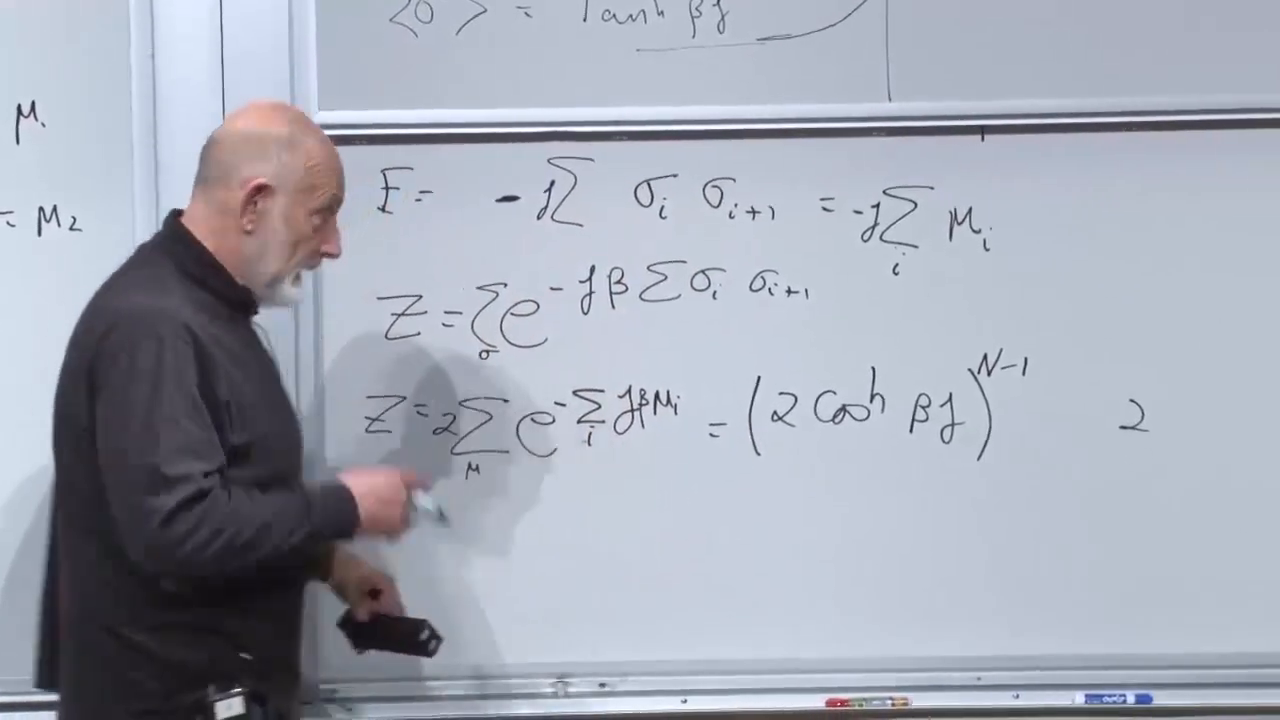
\includegraphics[width=0.82\textwidth]{lecture_09_figure_04.png}
\caption{将格点哈密顿量改写为对独立键的求和，以及由此得到的因子化配分函数。}
\lectureframe{00:35:35}
\end{figure}

\begin{classroomqa}
\audiencequestion{当最终答案变成幂时，指数中的求和到哪里去了？}
\lecturerresponse{它在变成幂之前先变成了乘积：
\[
e^{\beta J\sum_i\mu_i}=\prod_i e^{\beta J\mu_i}.
\]
对所有键构型的求和随后分解为每个键的一个两项求和。由于每个因子都是\(2\cosh(\beta J)\)，乘积就是它的\((N-1)\)次幂。写出三个自旋和两个键的情形，可以使因子化完全明确。\lecturetimestamp{00:33:25--00:35:36}}
\end{classroomqa}

这是一个简单的对偶描述：格点上的耦合变量已被替换为键上的非耦合变量。\emph{对偶}一词是恰当的，因为同一系统具有两种自由度看起来非常不同的描述。在这里，它是针对一维开链的一个精确变量替换。

用点阵的语言来说，原始变量生活在顶点上，而新变量生活在边上。第一个自旋的全局选择是从边重构顶点所需的唯一额外数据。这种格点—键的交换是这样一个模式的一个朴素例子，而该模式在高维统计力学中会变得强大得多。

\subsection{最近邻保真度}

每个键都有相同的分布，
\begin{equation}
\begin{aligned}
\Pr(\mu=+1)&=\frac{e^{\beta J}}{2\cosh(\beta J)},\\
\Pr(\mu=-1)&=\frac{e^{-\beta J}}{2\cosh(\beta J)}.
\end{aligned}
\end{equation}
因此，
\begin{equation}
\expect{\mu_i}
=\expect{\sigma_i\sigma_{i+1}}
=\tanh(\beta J).
\label{eq:nearest-correlation}
\end{equation}

\begin{figure}[ht]
\centering
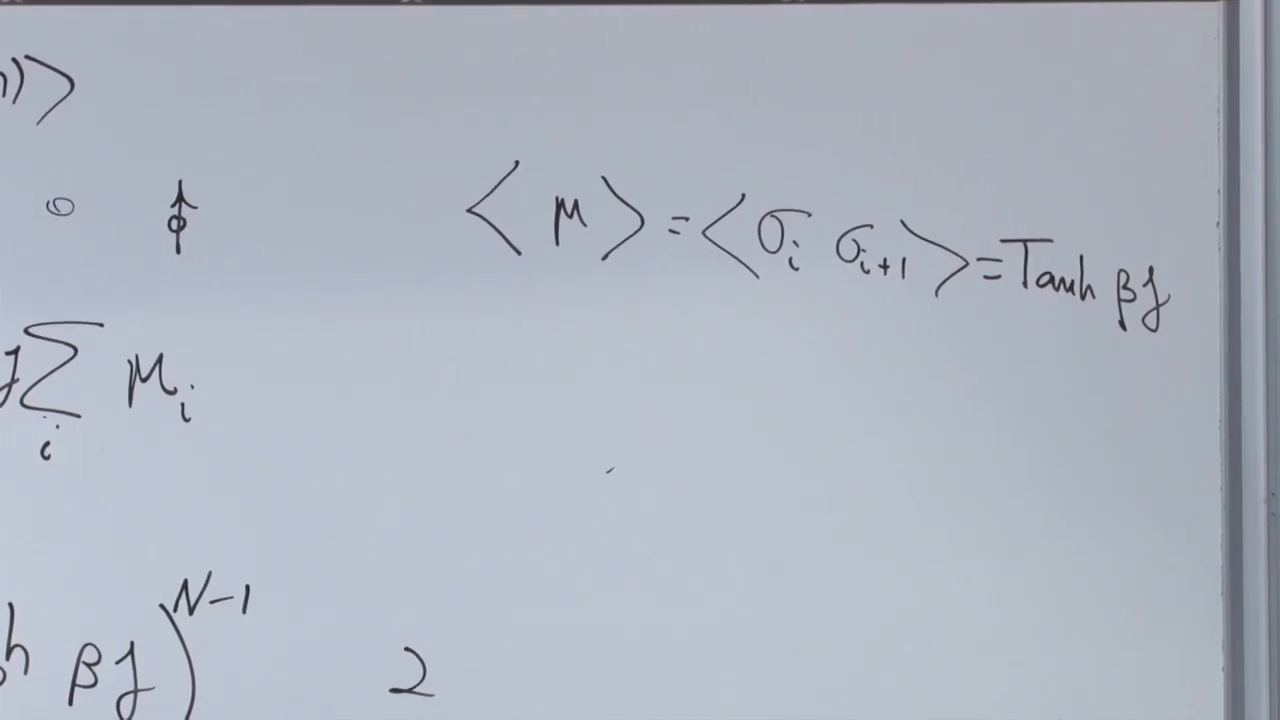
\includegraphics[width=0.80\textwidth]{lecture_09_figure_05.png}
\caption{将最近邻关联表示为键变量的平均值。}
\lectureframe{00:36:52}
\end{figure}

因此，相邻自旋一致的概率为
\begin{equation}
p_{\rm same}
=\frac{1+\tanh(\beta J)}{2}.
\end{equation}
它在正\(J\)时超过二分之一，在零温度时趋于一，而在无穷大温度时变为二分之一。

\begin{classroomqa}
\audiencequestion{为什么正的最近邻关联意味着自旋倾向于同向排列而不是反向排列？}
\lecturerresponse{对于\(J>0\)，同向键的能量为\(-J\)，反向键的能量为\(+J\)。\(\expect{\mu}\)为正值说明\(\mu=+1\)，即同向排列，出现得更频繁。真实材料究竟具有铁磁还是反铁磁的有效耦合，取决于其微观电子结构；这里的符号约定描述的是铁磁体。\lecturetimestamp{00:43:45--00:44:48}}
\end{classroomqa}

\begin{classroomqa}
\audiencequestion{在非常高的温度下，这个关联会怎样？}
\lecturerresponse{当\(T\to\infty\)时，\(\beta\to0\)，且\(\tanh(\beta J)\to0\)。此时即使最近邻之间也不携带关于彼此的任何信息：每个自旋实际上都是随机猜测。\lecturetimestamp{00:46:42--00:47:20}}
\end{classroomqa}

\subsection{长程关联}

对于相隔\(r\)个键的自旋，
\begin{align}
\sigma_i\sigma_{i+r}
&=\sigma_i
\left(\prod_{k=i+1}^{i+r-1}\sigma_k^2\right)
\sigma_{i+r}\\
&=(\sigma_i\sigma_{i+1})
(\sigma_{i+1}\sigma_{i+2})\cdots
(\sigma_{i+r-1}\sigma_{i+r})\\
&=\prod_{k=i}^{i+r-1}\mu_k.
\end{align}
由于\(\mu_k\)相互独立，
\begin{equation}
C(r)=\expect{\sigma_i\sigma_{i+r}}
=\left[\tanh(\beta J)\right]^r.
\label{eq:exact-correlation}
\end{equation}

\begin{figure}[ht]
\centering
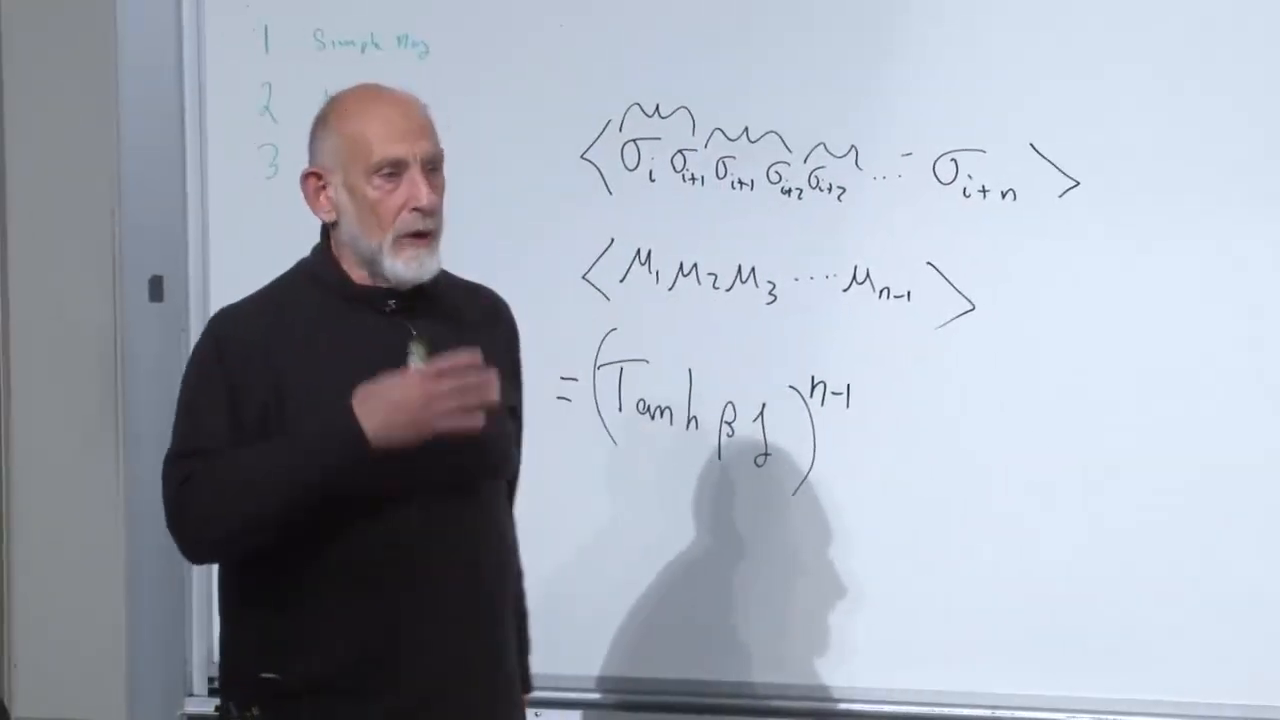
\includegraphics[width=0.80\textwidth]{lecture_09_figure_06.png}
\caption{中间的\(\sigma_k^2=1\)因子将远端自旋的乘积转化为独立键的乘积。}
\lectureframe{00:41:35}
\end{figure}

\begin{classroomqa}
\audiencequestion{关联函数只包含两个端点自旋。那么所有中间自旋是从哪里来的？}
\lecturerresponse{它们只是作为等于1的因子被插入：\(\sigma_k^2=1\)。将相邻的副本配对，就把端点乘积转化为键变量，而这些正是其热分布可因式分解的变量。关联函数的值并未改变。\lecturetimestamp{00:41:41--00:42:26}}
\end{classroomqa}

在任意有限温度下，
\begin{equation}
0<\tanh(\beta J)<1,
\end{equation}
因此记忆呈指数衰减。写出
\begin{equation}
C(r)=e^{-r/\xi}
\end{equation}
即定义了精确的关联长度
\begin{equation}
\xi^{-1}=-\log\!\left[\tanh(\beta J)\right].
\label{eq:correlation-length}
\end{equation}
只有在\(T=0\)时，\(\xi\)才发散。在低但非零的温度下，
\begin{equation}
\xi\simeq \frac{1}{2}e^{2\beta J},
\end{equation}
因此链中可以包含非常长的同向排列段，却不具有真正的无限程有序。

因此这条链看起来是成团的。人们看到一长串自旋向上，然后一次翻转，接着一长串自旋向下，然后再一次翻转。低温使这些串变长，因为畴壁很稀少；它并不会完全消除畴壁。磁化需要无限长的记忆长度，而不仅仅是很大的记忆长度。

\section{为什么更多邻居会改变问题}

一维不提供任何纠错能力。一旦某个键与其前驱不一致，下一个自旋就没有独立的信息来源告诉它原本意图是哪个取向。因此这条链由被偶尔翻转隔开的长同向排列畴组成。

在正方点阵中，每个格点有四个最近邻。在立方点阵中，它有六个。在\(d\)维超立方点阵中，它有
\begin{equation}
z=2d
\end{equation}
个最近邻。一个格点若收到三条一致的信息和一条不一致的信息，就可以遵从多数。多邻居环境抑制孤立错误的方式，与冗余信息实现纠错的方式大致相同。

如果邻居的平均自旋为\(m\)，则它们的和具有平均值\(zm\)。其普通涨落量级为\(\sqrt{z}\)，因此在远离\(m=0\)处，相对涨落大致按如下方式标度：
\begin{equation}
\frac{\sqrt{z}}{z|m|}
=\frac{1}{\sqrt{z}\,|m|}.
\end{equation}
这就是为什么在大的配位数下平均场变得可信。它也提醒我们，在临界点附近\(m\)很小，该近似最不可靠。

一句被记住的谚语抓住了大数直觉：一百张独立的选票不太可能全都朝同一方向出错。其定量版本就是平方根定律。\(z\)个变量中的相干偏置正比于\(z\)，而随机不一致通常只正比于\(\sqrt{z}\)。因此，增大维度不仅改变邻居的数量，也改变它们集体信息的可靠性。

\begin{classroomqa}
\audiencequestion{高于三维的维度是否对应某种物理磁性材料？}
\lecturerresponse{不能直接作为空间维度来对应。大的\(d\)是一个可解极限，其中每个格点有许多邻居，平均化变得可控。一旦在那里看清了机制，就可以追问它在多大程度上能延续到物理维度。对于Ising模型，二维已经足以出现有限温度相变，尽管平均场并不能给出精确的二维答案。\lecturetimestamp{00:52:32--00:53:50}}
\end{classroomqa}

\section{作为自洽问题的平均场}

聚焦于一个自旋\(\sigma_i\)。它与它的\(z=2d\)个邻居的相互作用为
\begin{equation}
E_i=-J\sigma_i\sum_{j\in{\rm nn}(i)}\sigma_j.
\label{eq:local-energy}
\end{equation}
令
\begin{equation}
m=\expect{\sigma}
\end{equation}
表示每个自旋的均匀磁化。平均场将涨落的邻居和替换为其平均值：
\begin{equation}
\sum_{j\in{\rm nn}(i)}\sigma_j
\longrightarrow zm=2dm.
\end{equation}
于是这个被选定的自旋具有有效的单自旋能量
\begin{equation}
E_i^{\rm MF}=-2dJm\,\sigma_i.
\label{eq:mean-field-energy}
\end{equation}

\begin{figure}[ht]
\centering
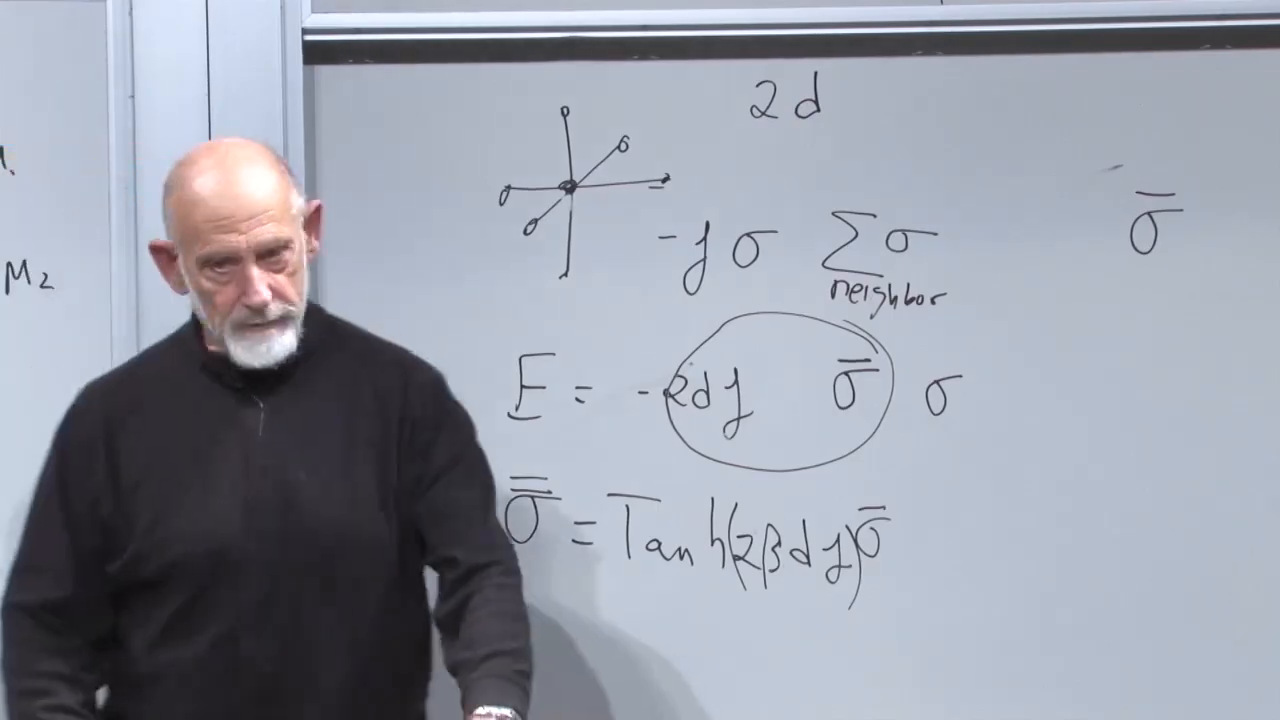
\includegraphics[width=0.82\textwidth]{lecture_09_figure_07.png}
\caption{一个选定的自旋、它的\(2d\)个最近邻，以及用平均磁化强度替换它们的和。}
\lectureframe{01:00:30}
\end{figure}

现在可以用有效场\(2dJm\)重新使用单自旋的结果：
\begin{equation}
\expect{\sigma_i}_{\rm effective}
=\tanh(2\beta dJm).
\end{equation}
但所选格点并不特殊。平移不变性要求它的平均值等于所假设的平均值\(m\)。因此
\begin{equation}
\boxed{m=\tanh(2\beta dJm)}.
\label{eq:self-consistency}
\end{equation}
这就是为什么平均场也称为自洽场近似：产生有效场的磁化强度必须等于由该场产生的磁化强度。

\begin{classroomqa}
\audiencequestion{有效单自旋答案中是否缺少一个\(\beta\)因子？}
\lecturerresponse{它必须存在。指数或双曲正切的宗量是无量纲的，因此有效能量\(2dJm\)表现为\(2\beta dJm\)。\lecturetimestamp{01:00:13--01:00:27}}
\end{classroomqa}

\begin{classroomqa}
\audiencequestion{这个方程只是说\(m\)与自身成正比吗？}
\lecturerresponse{不是。未知的磁化强度出现在一个非线性函数内部：
\[
m=\tanh(2\beta dJm).
\]
这是一个隐式方程，可能有一个或几个解，取决于温度。\lecturetimestamp{01:02:12--01:02:42}}
\end{classroomqa}

\begin{classroomqa}
\audiencequestion{自洽方程是否假设高温或双曲正切的宗量很小？}
\lecturerresponse{不是。方程\(m=\tanh(2\beta dJm)\)是在每个温度下的完整平均场方程。只有像\(\tanh x\simeq x\)这样的后续近似才要求\(x\)很小，它被用于临界点附近以确定或展开新出现的解。\lecturetimestamp{01:02:44--01:03:12}}
\end{classroomqa}

\begin{classroomqa}
\audiencequestion{上划线记号与通常的尖括号平均不同吗？}
\lecturerresponse{不。黑板上使用的横线是热平均的简写：\(\bar{\sigma}=\expect{\sigma}=m\)。\lecturetimestamp{01:03:19--01:03:42}}
\end{classroomqa}

\begin{classroomqa}
\audiencequestion{这\(2d\)个自旋都是最近邻吗，更长程的耦合会有类似的效果吗？}
\lecturerresponse{在超立方点阵上，是的：沿\(d\)个坐标轴中的每一个都有两个最近邻。次近邻和更远距离的耦合是另一个模型，通常带有它们自己的强度，但增加相互作用范围也会提高有效配位数，并能使平均场推理更准确。\lecturetimestamp{01:03:43--01:05:12}}
\end{classroomqa}

\section{相变的图示}

定义
\begin{equation}
K=2\beta dJ,
\qquad
y=Km.
\end{equation}
则方程~\eqref{eq:self-consistency}变为
\begin{equation}
\frac{y}{K}=\tanh y.
\label{eq:graph-equation}
\end{equation}
右边是一个固定的S形函数。左边是一条过原点、斜率为
\begin{equation}
\frac{1}{K}=\frac{T}{2dJ},
\end{equation}
的直线，其中\(k_{\rm B}=1\)。

在高温下，这条直线很陡，只与\(\tanh y\)相交于\(y=0\)。在低温下，这条直线较平缓，有三个交点：\(y=0\)和一对对称的\(y=\pm y_0\)。阈值出现在直线与\(\tanh y\)在原点处斜率相同时。由于\(\tanh'(0)=1\)，
\begin{equation}
K_c=1,
\qquad
T_c^{\rm MF}=2dJ.
\label{eq:mean-field-tc}
\end{equation}
这是平均场临界温度，而不是低维中的精确答案。

假设\(J>0\)说明相邻自旋倾向于一致；它并不在\(+m\)与\(-m\)之间做出选择。在零外场下，哈密顿量在全局翻转\(\sigma_i\mapsto-\sigma_i\)下不变，因此两个非零交点在物理上等价。只取图的右半部分是一种方便的绘图约定，而不是丢失了负相。

\begin{figure}[ht]
\centering
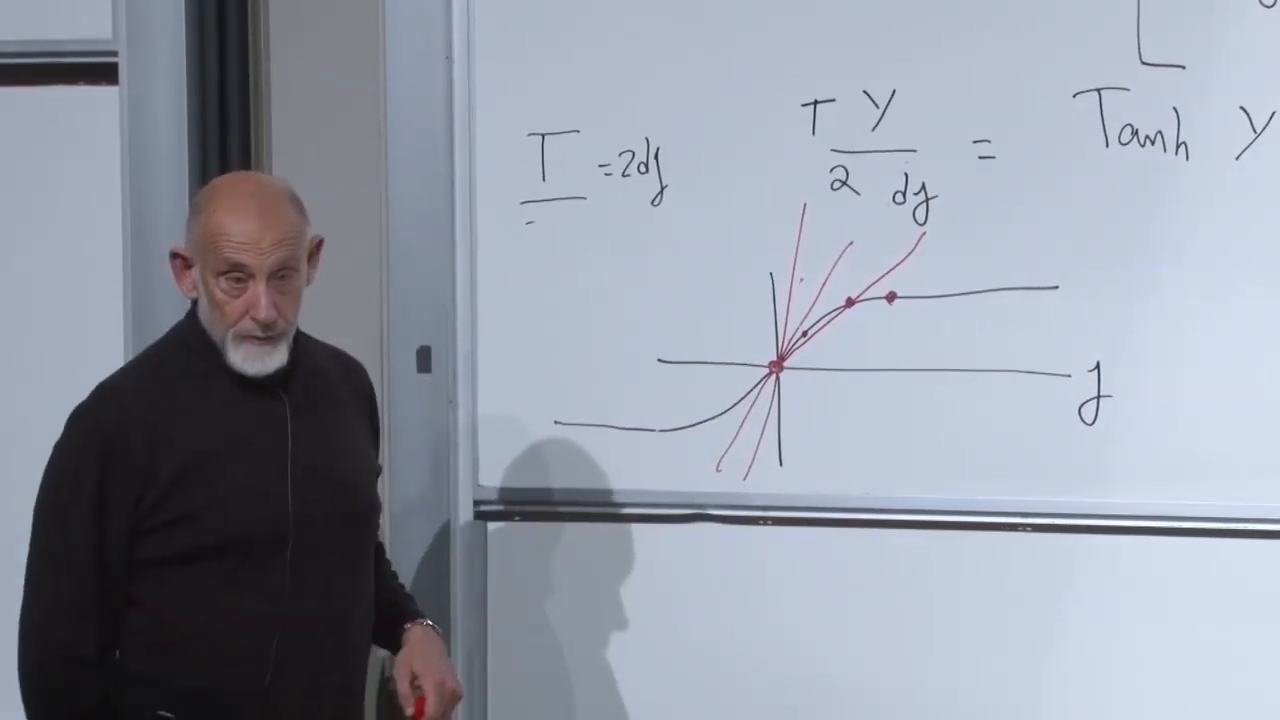
\includegraphics[width=0.82\textwidth]{lecture_09_figure_08.png}
\caption{直线族与\(\tanh y\)：一个高温交点与三个低温交点。}
\lectureframe{01:11:50}
\end{figure}

\begin{figure}[ht]
\centering
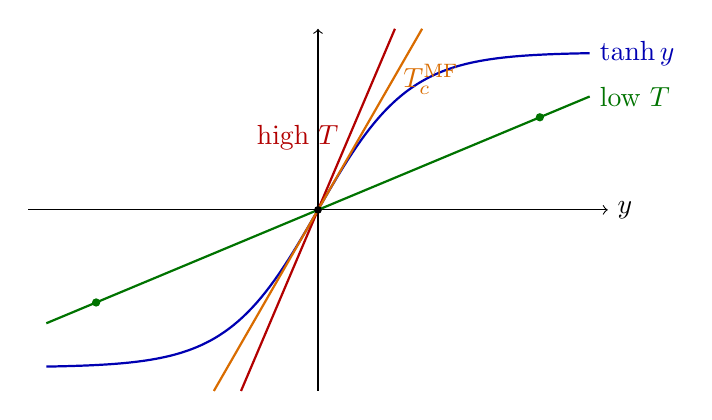
\begin{tikzpicture}[x=1.15cm,y=2.0cm]
\draw[->] (-3.2,0) -- (3.2,0) node[right] {$y$};
\draw[->] (0,-1.15) -- (0,1.15);
\draw[thick,blue!70!black,domain=-3:3,samples=120]
  plot (\x,{tanh(\x)}) node[right] {$\tanh y$};
\draw[thick,red!70!black] (-0.85,-1.15) -- (0.85,1.15)
  node[pos=0.70,left] {high \(T\)};
\draw[thick,orange!85!black] (-1.15,-1.15) -- (1.15,1.15)
  node[pos=0.86,right] {\(T_c^{\rm MF}\)};
\draw[thick,green!45!black] (-3,-0.72) -- (3,0.72)
  node[right] {low \(T\)};
\fill (0,0) circle (1.4pt);
\fill[green!45!black] (-2.45,-0.588) circle (1.5pt);
\fill[green!45!black] (2.45,0.588) circle (1.5pt);
\end{tikzpicture}
\caption{对图解法自洽论证的归一化重构。}
\end{figure}

非零分支连续地出现。在转变附近，
\begin{equation}
\tanh(Km)=Km-\frac{(Km)^3}{3}+O(m^5).
\end{equation}
对于\(K>1\)，小的非零解满足
\begin{equation}
m^2\simeq \frac{3(K-1)}{K^3}.
\end{equation}
因此平均场预言了熟悉的平方根式起始\(m\propto(T_c-T)^{1/2}\)。

稳定性陈述也可以不依赖于图的画法来给出。在相差一个与\(m\)无关的常数的意义下，每自旋的平均场自由能为
\begin{equation}
f_{\rm MF}(m)
=dJm^2-\frac{1}{\beta}
\log\!\left[2\cosh(2\beta dJm)\right].
\label{eq:mf-free-energy}
\end{equation}
其驻定条件为
\begin{equation}
\frac{\partial f_{\rm MF}}{\partial m}
=2dJ\left[m-\tanh(2\beta dJm)\right]=0.
\end{equation}
在\(T_c^{\rm MF}\)以上，\(m=0\)是最小值。在其以下，原点是局部极大值，而两个非零解是简并的最小值。交点的几何与自由能的热力学说的是同一件事。

\begin{classroomqa}
\audiencequestion{解\(m=0\)在\(T_c^{\rm MF}\)以下仍是一个交点。为什么非零分支应当是物理的？}
\lecturerresponse{从零温开始将系统向上移动，已经把它置于一个磁化分支上。更形式化地说，在转变温度以下，平均场自由能在\(\pm m_0\)处有极小值，而\(m=0\)则成为极大值。于是无穷小的外场会选中一个极小值，并消除表面上的歧义。\lecturetimestamp{01:11:34--01:12:18}}
\end{classroomqa}

\section{为什么一维会击败平均场}

将\(d=1\)代入方程~\eqref{eq:mean-field-tc}会预言在\(T=2J\)处发生转变，这与精确的一维解相矛盾。并没有任何代数量发散。该近似之所以失败，是因为两个近邻并不构成一个大的统计热浴，也因为一维畴壁带有异常的熵。

从全向上的态出发。一个断键将其能量从\(-J\)变为\(+J\)，因此每个断键的代价为
\begin{equation}
\Delta E_{\rm bond}=2J.
\end{equation}
在正方点阵上，一个翻转的自旋断开四个键，代价为\(8J\)。两个相邻的翻转自旋具有六个断键的周长，代价为\(12J\)，而两个相距很远的翻转则断开八个键，代价为\(16J\)。

\begin{figure}[ht]
\centering
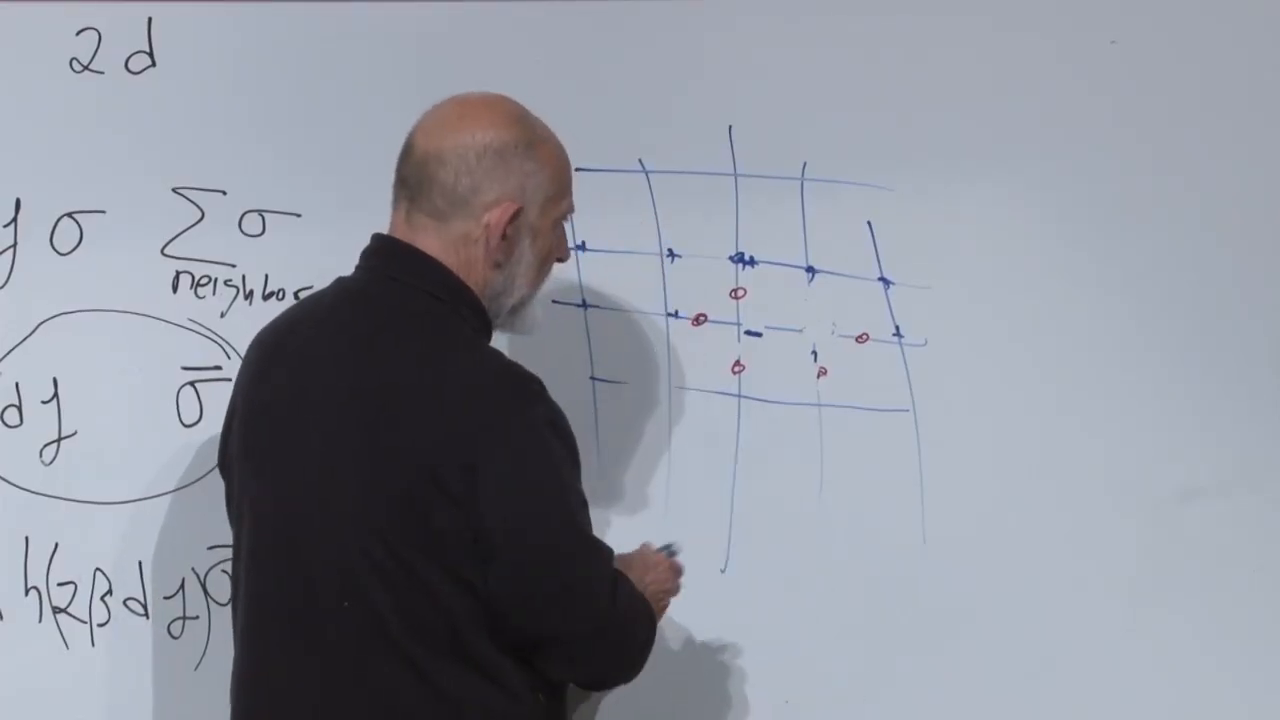
\includegraphics[width=0.82\textwidth]{lecture_09_figure_09.png}
\caption{正方点阵中两个相邻的反向自旋；它们共享的键得到满足，留下六键边界。}
\lectureframe{01:17:30}
\end{figure}

因此在二维中，一个紧凑的反向液滴所付出的能量正比于其边界长度：
\begin{equation}
\Delta E_{\rm 2d}=2J\,|\partial D|.
\end{equation}
使液滴长大通常也会使其边界长大。

一维则不同。一个连续的反向块，无论多长，都只有两个畴壁：
\begin{equation}
\Delta E_{\rm 1d}=2(2J)=4J.
\label{eq:one-d-domain-cost}
\end{equation}

\begin{figure}[ht]
\centering
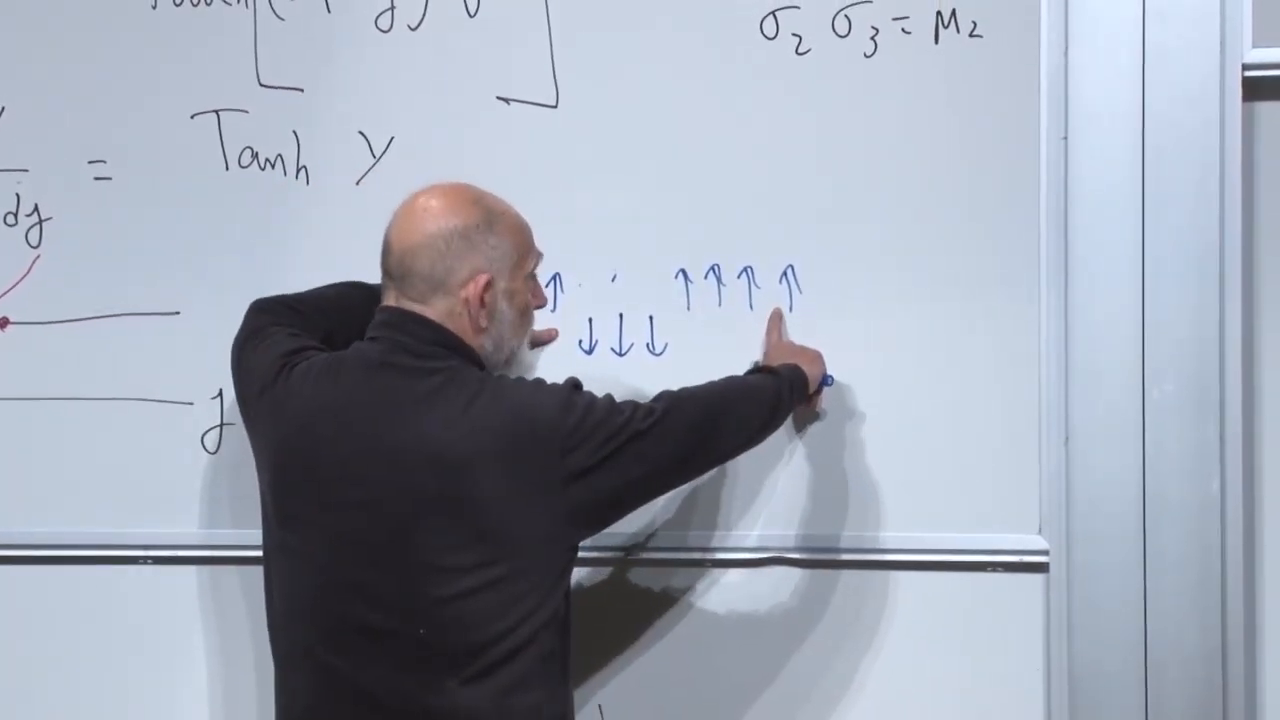
\includegraphics[width=0.82\textwidth]{lecture_09_figure_10.png}
\caption{一维中一个长反向块仅由两个畴壁界定。}
\lectureframe{01:19:10}
\end{figure}

在一条有\(N\)个格点的链中，选择这样一个块的两个壁的方式有\(N^2\)量级种。它们的能量并不随两壁之间间距的增大而增大。因此在任何正温度下，熵都会提供任意大的反向畴。在二维中，边界能量在足够低的温度下可以战胜轮廓熵。这种能量—熵竞争正是平均场在把\(d=1\)和\(d=2\)仅仅当作同一系数的不同数值处理时所看不到的几何事实。

\begin{classroomqa}
\audiencequestion{恒定的双壁代价是否要求翻转的自旋彼此相邻？}
\lecturerresponse{是的。该论断针对的是一个连续的反向块。如果翻转的自旋形成若干个分离的块，那么每个块都会引入两个额外的畴壁。要点在于，单个块可以任意长，却仍然只保留两个壁。\lecturetimestamp{01:18:32--01:18:40}}
\end{classroomqa}

\begin{classroomqa}
\audiencequestion{平均场方程本身似乎并未显示出\(d=1\)与\(d=2\)之间的定性区别。问题就在这里吗？}
\lecturerresponse{正是如此。平均场对每一个正的\(d\)都预言存在转变，因此它在一维中是定性错误的。它的推导假定了许多弱涨落的近邻，并丢弃了畴壁几何。决定一维情形的是精确的键解，而不是平均场替换\(d=1\)。\lecturetimestamp{01:19:44--01:20:28}}
\end{classroomqa}

\section{外场选择相}

加入一个均匀场\(h\)，约定\(h>0\)有利于\(\sigma=+1\)：
\begin{equation}
H=-J\sum_{\langle ij\rangle}\sigma_i\sigma_j
-h\sum_i\sigma_i.
\label{eq:ising-with-field}
\end{equation}
一个选定自旋的平均场能量为
\begin{equation}
E_i^{\rm MF}=-(2dJm+h)\sigma_i,
\end{equation}
而自洽方程变为
\begin{equation}
\boxed{m=\tanh\!\left[\beta(2dJm+h)\right]}.
\label{eq:self-consistency-field}
\end{equation}
取\(K=2\beta dJ\)和\(y=Km\)，
\begin{equation}
\frac{y}{K}=\tanh(y+\beta h).
\label{eq:shifted-graph}
\end{equation}

\begin{figure}[ht]
\centering
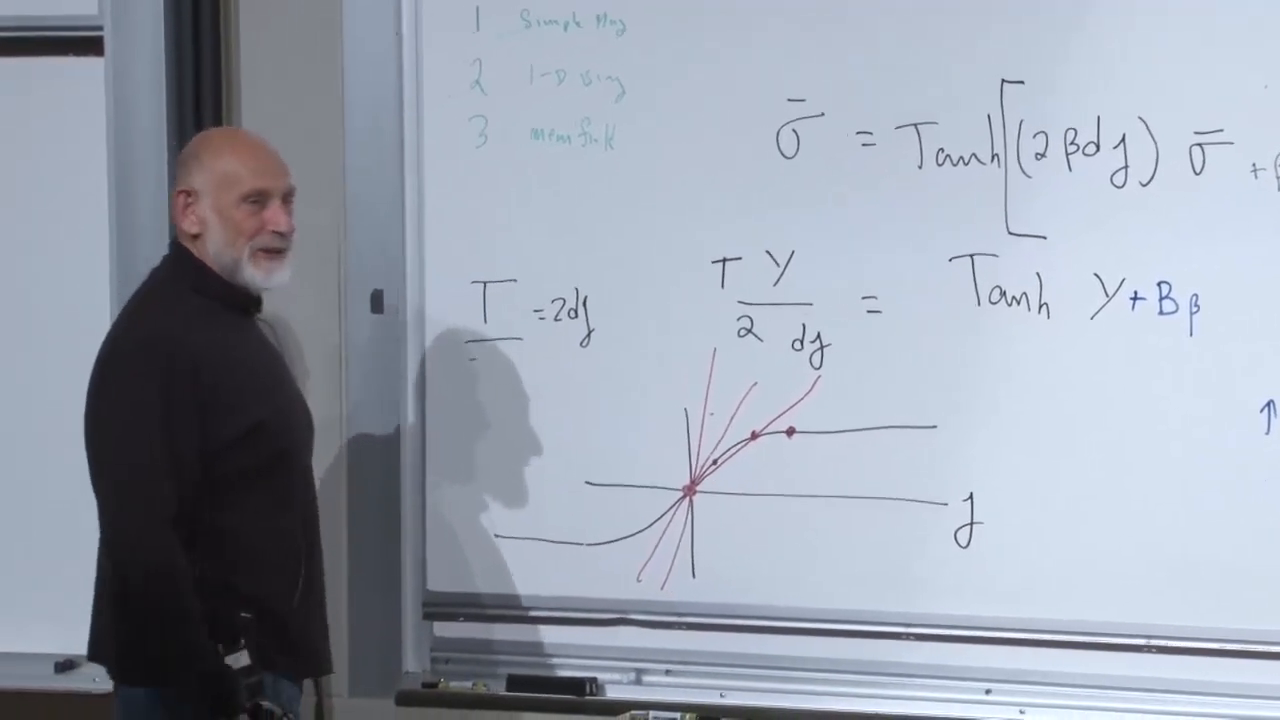
\includegraphics[width=0.82\textwidth]{lecture_09_figure_11.png}
\caption{在自洽方程中加入的外场项，以及相应的平移后图解构造。}
\lectureframe{01:26:20}
\end{figure}

\begin{classroomqa}
\audiencequestion{为什么场只加在双曲正切内部？它是否也应当改变左边？}
\lecturerresponse{左边是假定的磁化强度\(m\)，或等价地\(y/K\)。右边是在总有效场\(2dJm+h\)中为一个自旋计算出的磁化强度。自洽性令这两个量相等。将\(y=Km\)作为定义保持不变，就把新项只放进了自变量\(\tanh(y+\beta h)\)中。\lecturetimestamp{01:23:46--01:26:18}}
\end{classroomqa}

\begin{classroomqa}
\audiencequestion{同样的图解变化能否通过移动直线而不是平移\(\tanh\)曲线来描述？}
\lecturerresponse{可以。人们可以保持\(\tanh y\)不变，并改写方程，使直线具有非零截距。交点完全相同。这两种描述的区别仅在于选择方程哪一边作为固定图形。\lecturetimestamp{01:35:07--01:36:26}}
\end{classroomqa}

对于\(h\neq0\)，原点不再是解。在\(T_c^{\rm MF}\)以下，任意小的正场选择正分支；负场选择负分支。

\begin{figure}[ht]
\centering
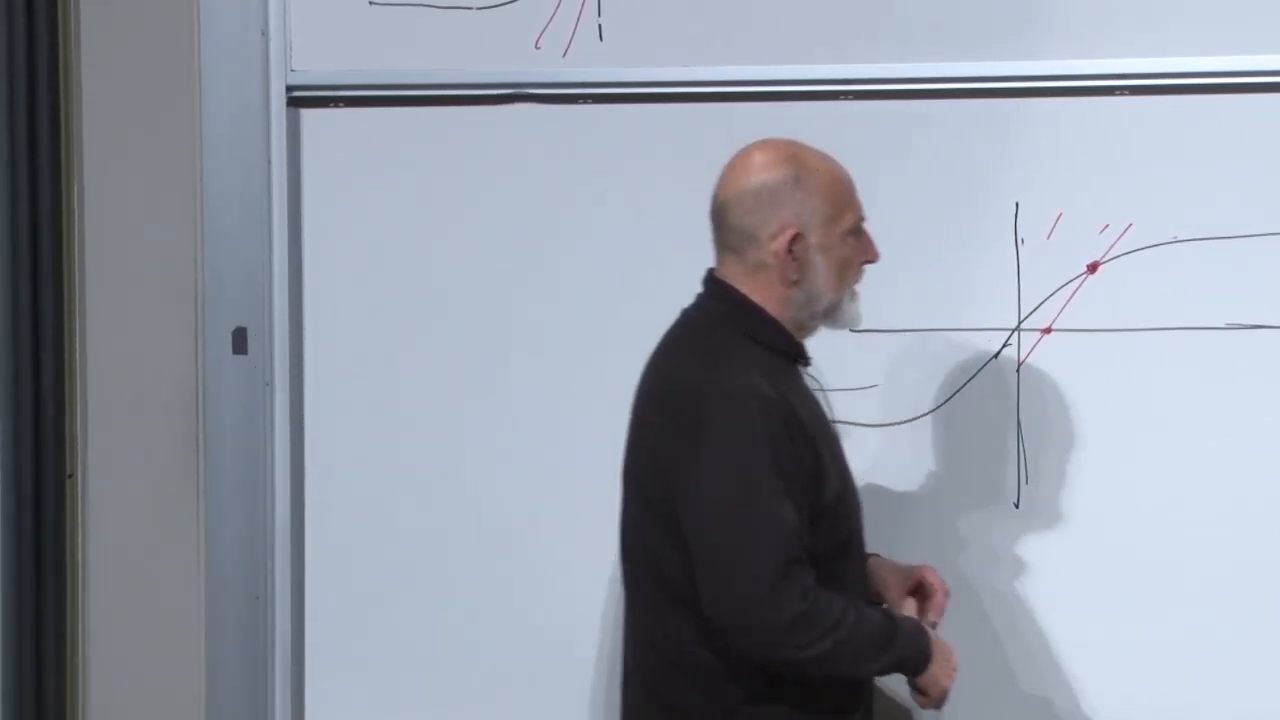
\includegraphics[width=0.82\textwidth]{lecture_09_figure_12.png}
\caption{弱场消除对称交点并选择一个磁化分支。}
\lectureframe{01:36:22}
\end{figure}

正确的陈述需要一个极限顺序。恰好处于\(h=0\)的有限系统具有自旋翻转对称性，因此在完整平衡系综中\(\expect{m}=0\)。自发磁化为
\begin{equation}
m_{\rm sp}
=\lim_{h\to0^+}\lim_{N\to\infty}\expect{m}_{N,h},
\end{equation}
其中热力学极限先取。反转无穷小场的符号给出\(-m_{\rm sp}\)。总场能差正比于\(Nh\)，因此即使极小的场对宏观样品也变得具有决定性。

相应的自由能使倾斜变得可见：
\begin{equation}
f_{\rm MF}(m;h)
=dJm^2-\frac{1}{\beta}
\log\!\left[2\cosh\!\left(\beta(2dJm+h)\right)\right].
\end{equation}
在\(h=0\)处，两个势阱深度相等。正的\(h\)降低正\(m\)势阱并升高负\(m\)势阱。每自旋的微扰可以很小，而总偏好乘以\(N\)后是宏观的。

\begin{classroomqa}
\audiencequestion{如果外场始终存在，磁化真的是自发的吗？}
\lecturerresponse{场仅用于选择分支。在固定\(T<T_c\)下，将系统取到无限大，然后令\(h\to0^+\)。即使选择场消失，磁化仍保持有限。反转极限符号选择相反的相。\lecturetimestamp{01:33:15--01:34:18}}
\end{classroomqa}

\begin{classroomqa}
\audiencequestion{在转变以下，零平均解实际上不可能，还是仅仅不稳定？}
\lecturerresponse{在恰好零场时，两个取向等权重的对称有限体积系综是可能的，且平均为零。失效的是它作为单一宏观相的稳定性。任意小的场改变广延能量平衡并选择一个取向；在热力学极限之后，所选磁化在场被移除时仍然存活。\lecturetimestamp{01:34:25--01:35:06}}
\end{classroomqa}

\begin{classroomqa}
\audiencequestion{在无限温度下，场偏置解会发生什么？}
\lecturerresponse{对于固定的有限\(h\)，当\(T\to\infty\)时，\(K=2\beta dJ\)和\(\beta h\)都趋于零。方程~\eqref{eq:self-consistency-field}于是给出\(m\to0\)。弱场选择低温分支，但它无法在无限热骚动下维持有序。\lecturetimestamp{01:27:39--01:29:51}}
\end{classroomqa}

\begin{classroomqa}
\audiencequestion{当温度和图的偏移一起变化时，如何确定交点去向何处？}
\lecturerresponse{隐式方程比移动的草图更可靠。在低温且\(h\)为正时，其稳定解趋近\(m=+1\)。在高温下，正切的展开给出
\[
m\simeq \beta(2dJm+h)
\quad\Longrightarrow\quad
m\simeq \frac{\beta h}{1-2\beta dJ},
\]
当\(\beta\to0\)时它趋于零。因此稳定分支将对齐的低温极限与弱极化的高温极限连接起来，而不会在转变以下停留在不稳定的原点。\lecturetimestamp{01:29:53--01:33:04}}
\end{classroomqa}

\section{磁反转是另一个问题}

\begin{classroomqa}
\audiencequestion{是什么使地球磁场反转方向？}
\lecturerresponse{这个问题超出了平衡伊辛模型的范围。地球主磁场由地球发电机产生：外核中导电流体的对流和旋转维持电流和磁场。反转是该非线性发电机的无规重组，而不是固态铁中的简单铁磁畴翻转。其详细时间过程不能由一个平衡序参量刻画，因此这里诚实的答案是伊辛计算并不解释触发机制。有用的联系只是一般性的：一个具有两个相反大尺度取向的系统可以在它们之间发生不稳定性。\footnote{参见\href{https://science.nasa.gov/science-research/earth-science/earths-magnetosphere-protecting-our-planet-from-harmful-space-energy/}{NASA关于地球发电机的概述}和\href{https://www.usgs.gov/programs/geomagnetism/introduction-geomagnetism}{USGS关于地磁学的介绍}。} \lecturetimestamp{01:38:39--01:40:32}}
\end{classroomqa}

精确链和平均场点阵现在给出两个截然不同的答案。在一维中，
\begin{equation}
\expect{\sigma_i\sigma_{i+r}}
=\left[\tanh(\beta J)\right]^r
\longrightarrow0
\qquad (T>0),
\end{equation}
因为有限能量的畴壁可以分隔任意长的反转区间。而在许多邻居的情况下，自洽场反而允许在
\begin{equation}
T_c^{\rm MF}=2dJ.
\end{equation}
以下存在稳定的非零解。这种对比不仅仅是代数上的。它是几何、能量、熵和冗余之间的竞争：一个错误能否自由传播，还是周围的点阵能够纠正它。
